Οι δύο προηγούμενες ενότητες περιγράφουν μεθόδους ελάττωσης (α) του σφάλματος
εκτίμησης προσανατολισμού όταν η εκτίμηση θέσης συμπίπτει με τη θέση του
αισθητήρα, και (β) του σφάλματος εκτίμησης θέσης όταν η εκτίμηση
προσανατολισμού ισούται με τον προσανατολισμό του αισθητήρα. Ωστόσο στη γενική
περίπτωση καμία ισότητα δεν ισχύει. Επιπρόσθετα, στη γενική περίπτωση
διαταραχές επηρεάζουν τις μετρήσεις του φυσικού αισθητήρα αποστάσεων και το
βαθμό ταύτισης του χάρτη $\bm{M}$ ως προς το περιβάλλον που αναπαριστά. Οι
τελευταίες δύο προτάσεις είναι κρίσιμης σημασίας για την από κοινού επίδοση των
μεθόδων που παρουσιάστηκαν στις προηγούμενες δύο ενότητες, λόγω των περιορισμών
της ενότητας \ref{subsection:02_04_02:07} και των παρατηρήσεων
\ref{rem:iterative} και \ref{remark:loc_prop_or}.


\subsection{Αντιμετώπιση των περιορισμών υπό γενικές συνθήκες}

Η παράκαμψη των επιδράσεων των περιορισμών που εμφανίζουν οι μέθοδοι
ευθυγράμμισης σε γενικές συνθήκες διαταραχών και ανισότητας στάσεων στοχεύει
στη λύση τεσσάρων ειδών προβλημάτων: Το πρώτο αφορά αποκλειστικά στη μέθοδο Πρώτων
Αρχών και περιγράφεται στο πρώτο σκέλος της Παρατήρησης
\ref{remark:02_04_02:02}. Το δεύτερο πρόβλημα αφορά στο δεύτερο σκέλος της
ίδιας παρατήρησης, και στην Παρατήρηση \ref{remark:02_04_02:03}. Το τέταρτο
πρόβλημα αφορά αποκλειστικά στη μέθοδο διόρθωσης θέσης, και συγκεκριμένα στην
Παρατήρηση \ref{remark:loc_prop_or}. Το τελευταίο αυτό πρόβλημα αποτελεί
ιδιότητα της μεθόδου ευθυγράμμισης θέσης, και η αντιμετώπισή του είναι συνέπεια
της λύσης των πρώτων δύο προβλημάτων.

Δεδομένου ότι όλες οι μέθοδοι εκτίμησης προσανατολισμού επηρεάζονται από την
έλλειψη μηχανισμού σύγκρισης εκτιμήσεων ως προς το σφάλμα τους, προσεγγίζουμε
τη λύση των δύο πρώτων προβλημάτων με τον ακόλουθο κοινό τρόπο.

Έστω ότι προσθέτουμε στη μέθοδο Πρώτων Αρχών την λειτουργία δειγματοληψίας του
χάρτη που παρουσιάστηκε στην ενότητα \ref{subsection:02_04_02:06}. Έστω επίσης
ότι αφαιρούμε από τη μέθοδο του Θησέα τη λειτουργία υπολογισμού και σύγκρισης
των τιμών της μετρικής Ποσοστού Διάκρισης για κάθε εκτιμώμενη εκτίμηση
προσανατολισμού. Τότε οι τρεις μέθοδοι γίνονται εναλλάξιμες υπό την έννοια ότι,
για μία δεδομένη εκτίμησης στάσης και ένα δεδομένο βαθμό δειγματοληψίας $\nu$,
καθεμία παράγει ένα σύνολο εκτιμήσεων στάσης μεγέθους $2^\nu$. Αυτό που
επιζητούμε σε αυτό το στάδιο είναι η εφεύρεση ενός μέτρου σύγκρισης των
εκτιμήσεων προσανατολισμού ως προς το (άγνωστο) σφάλμα τους. Το μέτρο σύγκρισης
θα πρέπει να αντικατοπτρίζει τις ιδιότητες

Τα κριτήρια που
πρέπει να ικανοποιεί αυτή η μετρική θα είναι, με βάση τα παραπάνω, τα ακόλουθα δύο:

\begin{itemize}
  \item Δεδομένης της παρατήρησης \ref{remark:loc_prop_or}, η μετρική θα πρέπει
        να αυξάνει για αυξανόμενο μέτρο σφάλματος προσανατολισμού και δεδομένο
        σφάλμα θέσης.
  \item Δεδομένης της παρατήρησης \ref{remark:02_04_02:01}, η μετρική θα πρέπει
        να αυξάνει για αυξανόμενο μέτρο σφάλματος θέσης και δεδομένο
        σφάλμα προσανατολισμού.
\end{itemize}


\begin{align}
  \text{CAER}_k \triangleq & \sum\limits_{n=0}^{N_s-1} \Bigg| \mathcal{S}_R[n] - \mathcal{S}_V[n]\Big|_{(\hat{x}_k, \hat{y}_k, \hat{\theta}_k)} \Bigg|
  \label{eq:caer}
\end{align}



\begin{figure}[h]\centering
  % GNUPLOT: LaTeX picture with Postscript
\begingroup
  \makeatletter
  \providecommand\color[2][]{%
    \GenericError{(gnuplot) \space\space\space\@spaces}{%
      Package color not loaded in conjunction with
      terminal option `colourtext'%
    }{See the gnuplot documentation for explanation.%
    }{Either use 'blacktext' in gnuplot or load the package
      color.sty in LaTeX.}%
    \renewcommand\color[2][]{}%
  }%
  \providecommand\includegraphics[2][]{%
    \GenericError{(gnuplot) \space\space\space\@spaces}{%
      Package graphicx or graphics not loaded%
    }{See the gnuplot documentation for explanation.%
    }{The gnuplot epslatex terminal needs graphicx.sty or graphics.sty.}%
    \renewcommand\includegraphics[2][]{}%
  }%
  \providecommand\rotatebox[2]{#2}%
  \@ifundefined{ifGPcolor}{%
    \newif\ifGPcolor
    \GPcolorfalse
  }{}%
  \@ifundefined{ifGPblacktext}{%
    \newif\ifGPblacktext
    \GPblacktexttrue
  }{}%
  % define a \g@addto@macro without @ in the name:
  \let\gplgaddtomacro\g@addto@macro
  % define empty templates for all commands taking text:
  \gdef\gplfronttext{}%
  \gdef\gplfronttext{}%
  \makeatother
  \ifGPblacktext
    % no textcolor at all
    \def\colorrgb#1{}%
    \def\colorgray#1{}%
  \else
    % gray or color?
    \ifGPcolor
      \def\colorrgb#1{\color[rgb]{#1}}%
      \def\colorgray#1{\color[gray]{#1}}%
      \expandafter\def\csname LTw\endcsname{\color{white}}%
      \expandafter\def\csname LTb\endcsname{\color{black}}%
      \expandafter\def\csname LTa\endcsname{\color{black}}%
      \expandafter\def\csname LT0\endcsname{\color[rgb]{1,0,0}}%
      \expandafter\def\csname LT1\endcsname{\color[rgb]{0,1,0}}%
      \expandafter\def\csname LT2\endcsname{\color[rgb]{0,0,1}}%
      \expandafter\def\csname LT3\endcsname{\color[rgb]{1,0,1}}%
      \expandafter\def\csname LT4\endcsname{\color[rgb]{0,1,1}}%
      \expandafter\def\csname LT5\endcsname{\color[rgb]{1,1,0}}%
      \expandafter\def\csname LT6\endcsname{\color[rgb]{0,0,0}}%
      \expandafter\def\csname LT7\endcsname{\color[rgb]{1,0.3,0}}%
      \expandafter\def\csname LT8\endcsname{\color[rgb]{0.5,0.5,0.5}}%
    \else
      % gray
      \def\colorrgb#1{\color{black}}%
      \def\colorgray#1{\color[gray]{#1}}%
      \expandafter\def\csname LTw\endcsname{\color{white}}%
      \expandafter\def\csname LTb\endcsname{\color{black}}%
      \expandafter\def\csname LTa\endcsname{\color{black}}%
      \expandafter\def\csname LT0\endcsname{\color{black}}%
      \expandafter\def\csname LT1\endcsname{\color{black}}%
      \expandafter\def\csname LT2\endcsname{\color{black}}%
      \expandafter\def\csname LT3\endcsname{\color{black}}%
      \expandafter\def\csname LT4\endcsname{\color{black}}%
      \expandafter\def\csname LT5\endcsname{\color{black}}%
      \expandafter\def\csname LT6\endcsname{\color{black}}%
      \expandafter\def\csname LT7\endcsname{\color{black}}%
      \expandafter\def\csname LT8\endcsname{\color{black}}%
    \fi
  \fi
    \setlength{\unitlength}{0.0500bp}%
    \ifx\gptboxheight\undefined%
      \newlength{\gptboxheight}%
      \newlength{\gptboxwidth}%
      \newsavebox{\gptboxtext}%
    \fi%
    \setlength{\fboxrule}{0.5pt}%
    \setlength{\fboxsep}{1pt}%
\begin{picture}(8400.00,4000.00)%
    \gplgaddtomacro\gplfronttext{%
    }%
    \gplgaddtomacro\gplfronttext{%
      \colorrgb{0.15,0.15,0.15}%
      \put(114,1003){\makebox(0,0)[r]{\strut{}$0.05$}}%
      \colorrgb{0.15,0.15,0.15}%
      \put(114,1571){\makebox(0,0)[r]{\strut{}$0.10$}}%
      \colorrgb{0.15,0.15,0.15}%
      \put(114,2137){\makebox(0,0)[r]{\strut{}$0.15$}}%
      \colorrgb{0.15,0.15,0.15}%
      \put(114,2705){\makebox(0,0)[r]{\strut{}$0.20$}}%
      \colorrgb{0.15,0.15,0.15}%
      \put(114,3273){\makebox(0,0)[r]{\strut{}$0.25$}}%
      \colorrgb{0.15,0.15,0.15}%
      \put(-700,600){\rotatebox{90}{\strut{}Σφάλμα θέσης $(\Delta x^2 + \Delta y^2)^{1/2}$}}%
      \colorrgb{0.15,0.15,0.15}%
      \put(253,111){\makebox(0,0){\strut{}$\small -\dfrac{\pi}{4}$}}%
      \colorrgb{0.15,0.15,0.15}%
      \put(1093,111){\makebox(0,0){\strut{}$\small -\dfrac{\pi}{8}$}}%
      \colorrgb{0.15,0.15,0.15}%
      \put(1513,111){\makebox(0,0){\strut{}$\small -\dfrac{\pi}{16}$}}%
      \colorrgb{0.15,0.15,0.15}%
      \put(1932,111){\makebox(0,0){\strut{}$\small 0.0$}}%
      \colorrgb{0.15,0.15,0.15}%
      \put(2351,111){\makebox(0,0){\strut{}$\small +\dfrac{\pi}{16}$}}%
      \colorrgb{0.15,0.15,0.15}%
      \put(2771,111){\makebox(0,0){\strut{}$\small +\dfrac{\pi}{8}$}}%
      \colorrgb{0.15,0.15,0.15}%
      \put(3611,111){\makebox(0,0){\strut{}$\small +\dfrac{\pi}{4}$}}%
      \colorrgb{0.15,0.15,0.15}%
      \put(1932,-360){\makebox(0,0){\strut{}Σφάλμα προσανατολισμού $\Delta\theta$}}%
    }%
    \gplgaddtomacro\gplfronttext{%
    }%
    \gplgaddtomacro\gplfronttext{%
      \colorrgb{0.15,0.15,0.15}%
      \put(4766,211){\makebox(0,0){\strut{}$0.05$}}%
      \colorrgb{0.15,0.15,0.15}%
      \put(5338,211){\makebox(0,0){\strut{}$0.10$}}%
      \colorrgb{0.15,0.15,0.15}%
      \put(5908,211){\makebox(0,0){\strut{}$0.15$}}%
      \colorrgb{0.15,0.15,0.15}%
      \put(6479,211){\makebox(0,0){\strut{}$0.20$}}%
      \colorrgb{0.15,0.15,0.15}%
      \put(7051,211){\makebox(0,0){\strut{}$0.25$}}%
      \colorrgb{0.15,0.15,0.15}%
      \put(5810,-360){\makebox(0,0){\strut{}Σφάλμα θέσης $(\Delta x^2 + \Delta y^2)^{1/2}$}}%
      \put(4000,2040){\rotatebox{90}{\makebox(0,0){\strut{}CAER [m]}}}%
    }%
    \gplgaddtomacro\gplfronttext{%
    }%
    \gplgaddtomacro\gplfronttext{%
    }%
    \gplgaddtomacro\gplfronttext{%
    }%
    \gplgaddtomacro\gplfronttext{%
      \colorrgb{0.00,0.00,0.00}%
      \put(8027,460){\makebox(0,0)[l]{\strut{} $0.0$}}%
      \colorrgb{0.15,0.15,0.15}%
      \put(8027,1100){\makebox(0,0)[l]{\strut{} $100.0$}}%
      \colorrgb{0.15,0.15,0.15}%
      \put(8027,1740){\makebox(0,0)[l]{\strut{} $200.0$}}%
      \colorrgb{0.15,0.15,0.15}%
      \put(8027,2379){\makebox(0,0)[l]{\strut{} $300.0$}}%
      \colorrgb{0.15,0.15,0.15}%
      \put(8027,3019){\makebox(0,0)[l]{\strut{} $400.0$}}%
      \colorrgb{0.15,0.15,0.15}%
      \put(8027,3659){\makebox(0,0)[l]{\strut{} $500.0$}}%
    }%
    \put(0,0){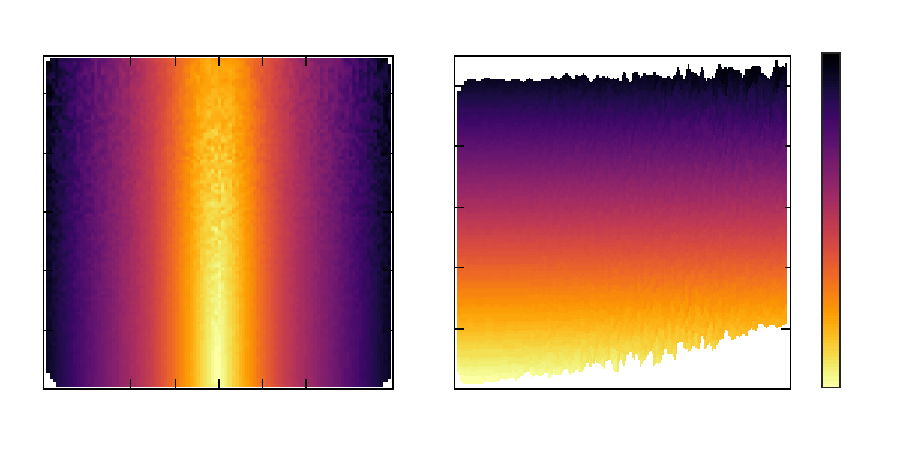
\includegraphics{./figures/parts/02/chapters/04/sections/04/caer_x2}}%
    \gplfronttext
  \end{picture}%
\endgroup

  \vspace{1cm}
  \caption{\small Κάτοψη (αριστερά) και πλάγια όψη (δεξιά) της μετρικής CAER
           (εξίσωση \ref{eq:caer}) από $10^6$ ζεύγη μίας σάρωσης σταθερής
           στάσης και εικονικών σαρώσεων που συλλήφθησαν από τυχαίες στάσεις,
           ανάλογα με την απόσταση $(\Delta x^2 + \Delta y^2)^{1/2}$ και το
           σχετικού προσανατολισμό $\Delta \theta$ των στάσεων από όπου αυτές
           καταγράφηκαν. Οι εκτιμήσεις στάσεις που είναι πιο κοντά στην
           πραγματική στάση από άποψη προσανατολισμού (α) παρουσιάζουν
           χαμηλότερες τιμές CAER από εκείνες που απέχουν περισσότερο από αυτήν
           και (β) παράγουν χαμηλότερα σφάλματα θέσης μόλις εισαχθούν στο
           Σύστημα Εκτίμησης Θέσης (Παρατήρηση \ref{remark:loc_prop_or})}
  \label{fig:02_04_04:caer}
\end{figure}




Επιπλέον το γενικό πρόβλημα ευθυγράμμισης
είναι πεπλεγμένο: το βέλτιστο σφάλμα προσανατολισμού δεν μπορεί να επιτευχθεί
όταν το σφάλμα θέσης δεν είναι μηδέν, και το βέλτιστο σφάλμα θέσης δεν μπορεί
να επιτευχθεί όταν το σφάλμα προσανατολισμού δεν είναι μηδέν (Παρατήρηση
\ref{rem:iterative}).


















\subsection{Το σύστημα από κοινού ευθυγράμμισης}


Σε αυτή την ενότητα παρουσιάζουμε το γενικό σύστημα που είναι ικανό να
ενσωματώσει τις τρεις μεθόδους ελάττωσης του σφάλματος εκτίμησης
προσανατολισμού και τη μέθοδο ελάττωσης του σφάλματος εκτίμησης θέσης.  Το
προτεινόμενο σύστημα μειώνει στην αρχή το πρώτο είδος σφάλματος, και στη
συνέχεια το δεύτερο. Ως συνέπεια της παρατήρησης \ref{rem:iterative}, η
διαδικασία επαναλαμβάνεται μέχρι την ικανοποίηση συνθήκης τερματισμού. Η
μέθοδος αυτή περιγράφεται στα ακόλουθα.


\begin{figure}[h]\centering
  

\tikzset{every picture/.style={line width=0.75pt}} %set default line width to 0.75pt

\begin{tikzpicture}[x=0.75pt,y=0.75pt,yscale=-0.5,xscale=0.5]
%uncomment if require: \path (0,1001); %set diagram left start at 0, and has height of 1001

%Flowchart: Decision [id:dp5485531374796404]
\draw[fill opacity=.25]  (240.5,167) -- (311.5,202) -- (240.5,237) -- (169.5,202) -- cycle ;
%Straight Lines [id:da5877536487984554]
\draw    (240.5,52.67) -- (240.5,108.67) ;
\draw [shift={(240.5,110.67)}, rotate = 270] [color={rgb, 255:red, 0; green, 0; blue, 0 }  ][line width=0.75]    (10.93,-3.29) .. controls (6.95,-1.4) and (3.31,-0.3) .. (0,0) .. controls (3.31,0.3) and (6.95,1.4) .. (10.93,3.29)   ;
%Straight Lines [id:da7274819726754627]
\draw    (240.5,237) -- (240.5,261.67) ;
\draw [shift={(240.5,263.67)}, rotate = 270] [color={rgb, 255:red, 0; green, 0; blue, 0 }  ][line width=0.75]    (10.93,-3.29) .. controls (6.95,-1.4) and (3.31,-0.3) .. (0,0) .. controls (3.31,0.3) and (6.95,1.4) .. (10.93,3.29)   ;
%Straight Lines [id:da7064477442798851]
\draw    (309.5,202) -- (382.5,202) -- (382.5,422) ;
\draw [shift={(382.5,423)}, rotate = 270.0] [color={rgb, 255:red, 0; green, 0; blue, 0 }  ][line width=0.75]    (10.93,-3.29) .. controls (6.95,-1.4) and (3.31,-0.3) .. (0,0) .. controls (3.31,0.3) and (6.95,1.4) .. (10.93,3.29)   ;
%Flowchart: Decision [id:dp1133428099178595]
\draw [ fill opacity=.25]  (240.5,266) -- (311.5,301) -- (240.5,336) -- (169.5,301) -- cycle ;
%Flowchart: Decision [id:dp5073654995853492]
\draw [ fill opacity=.25]  (239.5,422) -- (310.5,457) -- (239.5,492) -- (168.5,457) -- cycle ;
%Straight Lines [id:da1335991408375894]
\draw    (239.5,492) -- (239.5,533.67) ;
\draw [shift={(239.5,535.67)}, rotate = 270] [color={rgb, 255:red, 0; green, 0; blue, 0 }  ][line width=0.75]    (10.93,-3.29) .. controls (6.95,-1.4) and (3.31,-0.3) .. (0,0) .. controls (3.31,0.3) and (6.95,1.4) .. (10.93,3.29)   ;
%Straight Lines [id:da5471544644867792]
\draw    (234.5,82.67) -- (130.5,82.67) -- (130.5,517.33) ;
\draw [shift={(236.5,82.67)}, rotate = 180] [color={rgb, 255:red, 0; green, 0; blue, 0 }  ][line width=0.75]    (10.93,-3.29) .. controls (6.95,-1.4) and (3.31,-0.3) .. (0,0) .. controls (3.31,0.3) and (6.95,1.4) .. (10.93,3.29)   ;
%Straight Lines [id:da06493806045400974]
\draw    (310.5,457) -- (329,457.03) -- (332,457.03) ;
\draw [shift={(332,457)}, rotate = 539.01] [color={rgb, 255:red, 0; green, 0; blue, 0 }  ][line width=0.75]    (10.93,-3.29) .. controls (6.95,-1.4) and (3.31,-0.3) .. (0,0) .. controls (3.31,0.3) and (6.95,1.4) .. (10.93,3.29)   ;
%Straight Lines [id:da02699596164541651]
\draw    (240.5,137) -- (240.5,161.67) ;
\draw [shift={(240.5,163.67)}, rotate = 270] [color={rgb, 255:red, 0; green, 0; blue, 0 }  ][line width=0.75]    (10.93,-3.29) .. controls (6.95,-1.4) and (3.31,-0.3) .. (0,0) .. controls (3.31,0.3) and (6.95,1.4) .. (10.93,3.29)   ;
%Straight Lines [id:da5283272652442879]
\draw    (240.5,336) -- (240.5,360.67) ;
\draw [shift={(240.5,362.67)}, rotate = 270] [color={rgb, 255:red, 0; green, 0; blue, 0 }  ][line width=0.75]    (10.93,-3.29) .. controls (6.95,-1.4) and (3.31,-0.3) .. (0,0) .. controls (3.31,0.3) and (6.95,1.4) .. (10.93,3.29)   ;
%Straight Lines [id:da11468273552980146]
\draw    (239.5,392.33) -- (239.5,417) ;
\draw [shift={(239.5,419)}, rotate = 270] [color={rgb, 255:red, 0; green, 0; blue, 0 }  ][line width=0.75]    (10.93,-3.29) .. controls (6.95,-1.4) and (3.31,-0.3) .. (0,0) .. controls (3.31,0.3) and (6.95,1.4) .. (10.93,3.29)   ;
%Straight Lines [id:da44842589807001]
\draw    (169.5,301) -- (136,301) ;
\draw [shift={(134,300.67)}, rotate = 360] [color={rgb, 255:red, 0; green, 0; blue, 0 }  ][line width=0.75]    (10.93,-3.29) .. controls (6.95,-1.4) and (3.31,-0.3) .. (0,0) .. controls (3.31,0.3) and (6.95,1.4) .. (10.93,3.29)   ;
%Straight Lines [id:da5521661750319236]
\draw    (382,488.67) -- (382,517.33) -- (130.5,517.33) ;

% Text Node
\draw (161,113) -- (406,113) -- (406,138) -- (161,138) -- cycle  ;
\draw (164,116) node [anchor=north west][inner sep=0.75pt]   [align=center] {\tiny Σύστημα Άπαξ Εκτίμησης Στάσης};
% Text Node
\draw    (241.84, 37.33) circle [x radius= 24.75, y radius= 14.85]   ;
\draw (241.84,37.33) node   [align=left] {\tiny Start};
% Text Node
\draw (207,183) node [anchor=north west][inner sep=0.75pt]  [align=center] {\tiny Συνθήκες };
\draw (198,198) node [anchor=north west][inner sep=0.75pt]  [align=center] {\tiny επαναφοράς};
% Text Node
\draw (205,282) node [anchor=north west][inner sep=0.75pt]  [align=center] {\tiny Συνθήκες};
\draw (201,297) node [anchor=north west][inner sep=0.75pt]  [align=center] {\tiny σύγκλισης};
% Text Node
\draw    (334,427.67) -- (433,427.67) -- (433,487.67) -- (334,487.67) -- cycle  ;
\draw (341,431.67) node [anchor=north west][inner sep=0.75pt]  [align=center] {\tiny Παραγωγή};
\draw (341,445.67) node [anchor=north west][inner sep=0.75pt]  [align=center] {\tiny $\hat{\bm{p}}^\prime$ από $\hat{\bm{p}}$,};
\draw (341,468.67) node [anchor=north west][inner sep=0.75pt]  [align=center] {\tiny $\nu \leftarrow \nu_{\min}$};
% Text Node
\draw (324,182.33) node [anchor=north west][inner sep=0.75pt]   [align=left] {\tiny Y};
% Text Node
\draw (251,245.33) node [anchor=north west][inner sep=0.75pt]   [align=left] {\tiny N};
% Text Node
\draw    (218,366.67) -- (263,366.67) -- (263,392.67) -- (218,392.67) -- cycle  ;
\draw (221,371.67) node [anchor=north west][inner sep=0.75pt]   [align=center] {\tiny $\nu$++};
% Text Node
\draw (251,343.33) node [anchor=north west][inner sep=0.75pt]   [align=left] {\tiny Y};
% Text Node
\draw (252,74.57) node [anchor=north west][inner sep=0.75pt]   [align=left] {\tiny $\nu$, $\mathcal{S}_R$, $\bm{M}$, $\hat{\bm{p}}$};
% Text Node
\draw (205,436) node [anchor=north west][inner sep=0.75pt] [align=center] {\tiny Συνθήκες};
\draw (199,454) node [anchor=north west][inner sep=0.75pt] [align=center] {\tiny τερματισμού};
% Text Node
\draw    (239.93, 555.33) circle [x radius= 48.79, y radius= 14.85]   ;
\draw (239.93,555.33) node   [align=left] {\tiny Terminate};
% Text Node
\draw (147,276.33) node [anchor=north west][inner sep=0.75pt]   [align=left] {\tiny N};
% Text Node
\draw (251,399.33) node [anchor=north west][inner sep=0.75pt]   [align=left] {\tiny Y};
% Text Node
\draw (314,437.33) node [anchor=north west][inner sep=0.75pt]   [align=left] {\tiny N};
% Text Node
\draw (251,145.57) node [anchor=north west][inner sep=0.75pt]   [align=left] {\tiny $\hat{\bm{p}}^\prime$};
% Text Node
\draw (250,493.33) node [anchor=north west][inner sep=0.75pt]   [align=left] {\tiny Y};


\end{tikzpicture}


  \caption{\small Το διάγραμμα ροής του FSMSM. Η εκτέλεση αρχίζει με μια αρχική
           γωνιακό βαθμό δειγματοληψίας $\nu_{\min}$, η σάρωση που καταγράφεται
           από το αισθητήρα φυσικού εύρους $\mathcal{S}_R$, και ο χάρτης του
           περιβάλλοντος $\bm{M}$. Η αρχική εκτίμηση της στάσης παρέχεται από
           ένα φίλτρο παρακολούθησης κατά τη διάρκεια της ανίχνευσης της στάσης
           ή με τη μορφή μιας υπόθεσης κατά τη διάρκεια της συνολικής
           εντοπισμού. Η εσωτερική μέθοδος One-step Pose Correction (διόρθωση
           πόζας ενός βήματος) (εικ. \ref{fig:02_04_04:inner_system}) καλείται
           επαναληπτικά, ενημερώνοντας την πόζα εκτίμηση, μέχρι να επιτευχθεί
           ένας μέγιστος βαθμός γωνιακής δειγματοληψίας}
  \label{fig:02_04_04:outer_system}
\end{figure}

Έστω οι προϋποθέσεις του προβλήματος \ref{prob:02_04}, δηλαδή
η αρχική εκτίμηση εισόδου $\hat{\bm{p}}(\hat{x}, \hat{y}, \hat{\theta})$,
η πραγματική σάρωση $\mathcal{S}_R$, και ο χάρτης $\bm{M}$. Τότε
η μέθοδος ελάττωσης του συνολικού σφάλματος εκτίμησης στάσης που προτείνουμε,
την οποία ονομάζουμε Fourier Scan--to--Map-Scan Matching (FSMSM) και η οποία
παρουσιάζεται στο σχήμα \ref{fig:02_04_04:outer_system},---η μέθοδος μειώνει το
σφάλμα με την επαναληπτική εκτέλεση της διαδικασίας ελάττωσης σφάλματος ενός
βήματος (One-step Pose Correction, OPC---σχήμα \ref{fig:02_04_04:inner_system}),
μέχρι να ικανοποιηθεί ένα σύνολο συνθηκών τερματισμού. Η FSMSM ξεκινά με ένα
αρχικό βαθμό δειγματοληψίας του χάρτη $\nu$ = $\nu_{\min}$. Η εκτίμηση της
στάσης εισόδου επεξεργάζεται από την OPC, και η έξοδός της
$\hat{\bm{p}}^\prime$ εξετάζεται ως προς συνθήκες ανάκτησης και
σύγκλισης. Εάν η προκύπτουσα εκτίμηση στάσης βρεθεί εκτός του χάρτη $\bm{M}$
τότε δημιουργείται μια νέα εκτίμηση από την αρχική
εκτίμηση, και η διαδικασία επανεκιννεί. Εάν δεν παρατηρείται σημαντική
διόρθωση της εκτίμησης
$\|\hat{\bm{p}}^\prime-\hat{\bm{p}}\|_2 < \varepsilon_{\delta p}$, τότε ο
βαθμός δειγματοληψίας του χάρτη $\nu$ αυξάνεται. Η αύξησή του χρησιμεύει ως
μέσο μείωσης του σφάλματος προσανατολισμού και συνεπώς του σφάλματος εκτίμησης
θέσης (Παρατήρηση \ref{remark:loc_prop_or}). Διαφορετικά, η διαδικασία
διόρθωσης της στάσης σε ένα βήμα είναι η εξής επαναλαμβάνεται έως ότου δεν
παρατηρηθεί σημαντική διόρθωση. Η διαδικασία επαναλαμβάνεται έως ότου
επιτευχθεί ο μέγιστος βαθμός δειγματοληψίας χάρτη $\nu$ = $\nu_{\max}$, σε
οπότε το FSMSM τερματίζει εάν πληρούται μια τελική συνθήκη. Αυτή η τελική
συνθήκη διευκολύνει την αποφυγή τοπικών μεγίστων. Στην περίπτωση που αυτό το
συνθήκη δεν ικανοποιείται, δημιουργείται μια νέα πόζα και η διαδικασία
επαναφέρεται.

\begin{figure}[h]\centering
  \tikzset{every picture/.style={line width=0.75pt}} %set default line width to 0.75pt

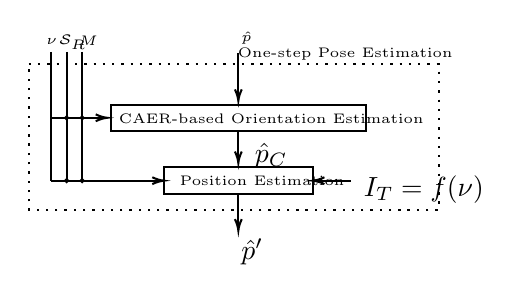
\begin{tikzpicture}[x=0.75pt,y=0.75pt,yscale=-0.5,xscale=0.5]
%uncomment if require: \path (0,542); %set diagram left start at 0, and has height of 542

\draw    (126.5,63) -- (126.5,187) ; % nu vertical
\draw    (141.5,63) -- (141.5,187) ; % S_R vertical line
\draw    (156.5,63) -- (156.5,187) ; % M vertical line
\draw    (307,64) -- (307,108) ; hat p vertical line

\draw [shift={(307,110)}, rotate = 270] [color={rgb, 255:red, 0; green, 0; blue, 0 }  ][line width=0.75]    (10.93,-3.29) .. controls (6.95,-1.4) and (3.31,-0.3) .. (0,0) .. controls (3.31,0.3) and (6.95,1.4) .. (10.93,3.29)   ; % hat p vertical arrow

\draw    (307,138.86) -- (307,167.86) ; % after caer based orientation box vertical line

\draw [shift={(307,169.86)}, rotate = 270] [color={rgb, 255:red, 0; green, 0; blue, 0 }  ][line width=0.75]    (10.93,-3.29) .. controls (6.95,-1.4) and (3.31,-0.3) .. (0,0) .. controls (3.31,0.3) and (6.95,1.4) .. (10.93,3.29)   ; % after caer based orientation box vertical arrow

\draw    (178.5,126.4) -- (156.5,126.4) ; % M horizontal line to CAER Based

\draw [shift={(156.5,126.4)}, rotate = 180] [color={rgb, 255:red, 0; green, 0; blue, 0 }  ][fill={rgb, 255:red, 0; green, 0; blue, 0 }  ][line width=0.75]      (0, 0) circle [x radius= 1.35, y radius= 1.35]   ; % M horizontal line to CAER based dot

\draw [shift={(180.5,126.4)}, rotate = 180] [color={rgb, 255:red, 0; green, 0; blue, 0 }  ][line width=0.75]    (10.93,-3.29) .. controls (6.95,-1.4) and (3.31,-0.3) .. (0,0) .. controls (3.31,0.3) and (6.95,1.4) .. (10.93,3.29)   ; % M horizontal arrow to caer based

\draw    (156.5,126.4) -- (141.5,126.4) ; % S_R horizontal line to caer based

\draw [shift={(141.5,126.4)}, rotate = 180] [color={rgb, 255:red, 0; green, 0; blue, 0 }  ][fill={rgb, 255:red, 0; green, 0; blue, 0 }  ][line width=0.75]      (0, 0) circle [x radius= 1.35, y radius= 1.35]   ; % S_R horizontal line to caer based dot

\draw    (141.5,126.4) -- (126.5,126.4) ; % nu to caer based line




\draw    (185.5,187) -- (126.0,187) ; % nu to S_R line to position estimation
\draw    (156.5,187) -- (141.5,187) ; % S_R to position estimation line
\draw    (235.0,187) -- (156.5,187) ; % M line to position estimation

\draw [shift={(156.5,187)}, rotate = 180] [color={rgb, 255:red, 0; green, 0; blue, 0 }  ][fill={rgb, 255:red, 0; green, 0; blue, 0 }  ][line width=0.75]      (0, 0) circle [x radius= 1.35, y radius= 1.35]   ; % M dot to position estimation
\draw [shift={(141.5,187)}, rotate = 180] [color={rgb, 255:red, 0; green, 0; blue, 0 }  ][fill={rgb, 255:red, 0; green, 0; blue, 0 }  ][line width=0.75]      (0, 0) circle [x radius= 1.35, y radius= 1.35]   ; % S_R dot to position estimation
\draw [shift={(235.0,187)}, rotate = 180] [color={rgb, 255:red, 0; green, 0; blue, 0 }  ][line width=0.75]    (10.93,-3.29) .. controls (6.95,-1.4) and (3.31,-0.3) .. (0,0) .. controls (3.31,0.3) and (6.95,1.4) .. (10.93,3.29)   ; % M arrow to position estimation



\draw (235,174) -- (379,174) -- (379,200) -- (235,200) -- cycle  ;
\draw (235,180) node [anchor=north west][inner sep=0.75pt]   [align=left] {\tiny \ \ Position Estimation};

\draw (425,179) node [anchor=north west][inner sep=0.75pt]   [align=left] {$I_T = f( \nu )$};
\draw (379,187) -- (415.5,187) ; % I = fn line to position estimation
\draw [shift={(379,187)}, rotate = 0] [color={rgb, 255:red, 0; green, 0; blue, 0 }  ][line width=0.75]    (10.93,-3.29) .. controls (6.95,-1.4) and (3.31,-0.3) .. (0,0) .. controls (3.31,0.3) and (6.95,1.4) .. (10.93,3.29)   ;% I = fn arrow to position estimation


\draw (320,147.5) node [anchor=north west][inner sep=0.75pt]   [align=left] {$\hat{\bm{p}}_{C}$};
\draw (307,240) node [anchor=north west][inner sep=0.75pt]   [align=left] {$\hat{\bm{p}}^{\prime }$};

\draw (307,200) -- (307,235) ; % p final vertical line
\draw [shift={(307,235)}, rotate = 270] [color={rgb, 255:red, 0; green, 0; blue, 0 }  ][line width=0.75]    (10.93,-3.29) .. controls (6.95,-1.4) and (3.31,-0.3) .. (0,0) .. controls (3.31,0.3) and (6.95,1.4) .. (10.93,3.29)   ; % p final vertical arrow



%Shape: Rectangle [id:dp8185193791005427]
\draw  [dash pattern={on 0.84pt off 2.51pt}] (105,75) -- (500,75) -- (500,215) -- (105,215) -- cycle ;
\draw (410,65) node  {\tiny One-step Pose Estimation};

% Text Node
\draw    (184,114) -- (430,114) -- (430,139) -- (184,139) -- cycle  ;
\draw (189,120) node [anchor=north west][inner sep=0.75pt]   [align=left] {\tiny CAER-based Orientation Estimation};
% Text Node
\draw (119,47) node [anchor=north west][inner sep=0.75pt]   [align=left] {\tiny \tiny $\nu$};
% Text Node
\draw (131,44) node [anchor=north west][inner sep=0.75pt]   [align=left] {\tiny $\mathcal{S}_{R}$};
% Text Node
\draw (307,40.57) node [anchor=north west][inner sep=0.75pt]   [align=left] {\tiny $\hat{\bm{p}}$};
% Text Node
\draw (150,44.57) node [anchor=north west][inner sep=0.75pt]   [align=left] {\tiny $\bm{M}$};


\end{tikzpicture}

  \caption{\small  βασική μέθοδος ευθυγράμμισης πόζας του FSMSM, που ονομάζεται
           One-step Pose Correction}
  \label{fig:02_04_04:inner_system}
\end{figure}


Δεδομένης μιας εκτίμησης πόζας εισόδου $\hat{\bm{p}}(\hat{x}, \hat{y},
\hat{\theta})$, η πραγματική σάρωση $\mathcal{S}_R$, ο χάρτης $\bm{M}$ και ένας
βαθμός δειγματοληψίας $\nu$, το σύστημα διόρθωσης πόζας ενός βήματος υπολογίζει
πρώτα εκτιμήσεις πόζας $2^\nu$ $\hat{\bm{P}}_{OC} = \{(\hat{x}, \hat{y},
\hat{\theta}_k)\}$, $k = 0,\dots,2^\nu$$-$$1$. Το σύστημα διόρθωσης
προσανατολισμού χρησιμοποιεί τον αλγόριθμο \ref{alg:algorithm_ufrcnu}. Η
λειτουργία του συμβολίζεται στο σχήμα.  \ref{fig:02_04_04:inner_system} με τον τελεστή
OC$(\cdot)$.

Τώρα, εάν η θέση της εκτίμησης της πόζας εισόδου συμπίπτει με τη θέση του του
πραγματικού αισθητήρα, η μετρική Percent Discrimination (εξ. \ref{eq:pd}) θα
αρκούσε για να χρησιμεύσει ως ακριβής προσδιοριστής της εκτίμησης της πόζας με
τον ελάχιστο σφάλμα προσανατολισμού. Στην πράξη, ωστόσο, η κατάταξη που
παρέχεται από την Percent Discrimination μετρική, μπερδεύεται από την ασυνέπεια
των δύο θέσεων.  Προκειμένου να αμβλυνθεί αυτό το φαινόμενο, κάθε εκτίμηση
στάσης στο $\hat{\bm{P}}_{OC}$ δίνεται στο σύστημα διόρθωσης θέσης, όπου η θέση
κάθε εκτίμησης πόζας μετατοπίζεται μία φορά ($I$=$1$), σύμφωνα με την
Αλγόριθμος \ref{alg:algorithm_icte}. Αυτή η λειτουργία, που συμβολίζεται με τον
τελεστή RPC$(\cdot)$ στην εικ. \ref{fig:02_04_04:inner_system}, παράγει το σύνολο
$\hat{\bm{P}}_{RPC} = \{(\hat{x}_k, \hat{y}_k, \hat{\theta}_k)\}$,
$|\hat{\bm{P}}_{RPC}| = 2^\nu$.  Ο σκοπός αυτής της πράξης είναι να να παρέχει
μια εκ των προτέρων εικόνα του επόμενου βήματος της διόρθωσης της θέσης: το
λιγότερο περιστροφικά κακή ευθυγράμμιση είναι μια εκτίμηση της στάσης, τόσο
λιγότερο θα αποκλίνει ως προς την προσανατολισμού και συνεπώς της θέσης σε
σχέση με την πραγματική θέση του αισθητήρα μόλις εισάγεται στο σύστημα
διόρθωσης θέσης (παρατήρηση \ref{remark:loc_prop_or}). Αυτή η απόκλιση
αποτυπώνεται από το αθροιστικό απόλυτο σφάλμα ανά ακτίνα (CAER) μετρική:
\begin{align}
  \text{CAER}_k = & \sum\limits_{n=0}^{N_s-1} \Bigg| \mathcal{S}_R[n] - \mathcal{S}_V[n]\Big|_{(\hat{x}_k, \hat{y}_k, \hat{\theta}_k)} \Bigg|
  \label{eq:caer}
\end{align}
όπου $k$ = $0,\dots,2^\nu$$-$$1$. Η μετρική CAER (εικ. \ref{fig:02_04_04:caer})
κωδικοποιεί ταυτόχρονα ένα βαθμό ευθυγράμμισης της θέσης και του
προσανατολισμού μεταξύ των δύο σαρώσεων εισόδου της.\footnote{Αντίθετα, η
αφαίρεση της απόλυτης τιμής θα παρείχε μόνο μια μετρική ευθυγράμμισης θέσης.}
Με την επανάληψη του διόρθωση θέσης κάθε εκτίμησης της θέσης στο
$\hat{\bm{P}}_{OC}$ και την καταγραφή την CAER για κάθε μια από τις
μετατοπισμένες εκτιμήσεις πόζας στο $\hat{\bm{P}_{RPC}}$, είναι είναι δυνατόν
να καθοριστεί μια κατάταξη σφάλματος πόζας μεταξύ των εκτιμήσεων πόζας στο
$\hat{\bm{P}}_{OC}$ και ταυτόχρονα να διατηρείται μόνο μία εκτίμηση πόζας για
την την επόμενη επανάληψη της μεθόδου διόρθωσης πόζας ενός
βήματος.\footnote{Αλλιώς, η διόρθωση της θέσης των εκτιμήσεων πόζας $2^\nu$ και
η επανατροφοδότησή τους στην διόρθωση πόζας ενός βήματος θα προκαλούσε εκθετικό
κόστος σε χρόνο εκτέλεσης.} Η εκτίμηση πόζας $\hat{\bm{p}}_C \in
\hat{\bm{P}}_{OC}$ η οποία, όταν μεταφράζεται μία φορά, καταγράφει το ελάχιστο
CAER μεταξύ όλων των παρόμοια επεξεργασμένων πόζων εκτιμήσεις στο
$\hat{\bm{P}}_{OC}$ εισάγεται στη μέθοδο διόρθωσης θέσης proper. Ο αριθμός των
επαναλήψεων μετάφρασης $I$ που υφίσταται είναι ένας αυξανόμενος συνάρτηση του
βαθμού δειγματοληψίας του χάρτη $\nu$.\footnote{Η λογική της αλυσιδωτής
σύνδεσης του αριθμού των μεταφραστικών επαναλήψεων με το βαθμό δειγματοληψίας
του χάρτη $\nu$ είναι η ακόλουθη.  Δεδομένου ότι το σφάλμα προσανατολισμού
είναι αντιστρόφως ανάλογο με το $\nu$, σε χαμηλούς βαθμούς δειγματοληψίας
χάρτη, όταν το σφάλμα εκτίμησης θέσης είναι στο υψηλότερο, εάν ο αριθμός των
μεταφραστικών επαναλήψεων ήταν υψηλός, τότε η θέση εκτίμηση της θέσης θα ήταν
ευάλωτη σε απόκλιση. Επομένως, ο αριθμός των μεταφραστικών επαναλήψεων
διατηρείται χαμηλός στα αρχικά στάδια έτσι ώστε να υπάρχει ισορροπία μεταξύ της
μείωσης του σφάλματος θέσης και της απόκλισης θέσης. Σε υψηλότερα τιμές του
$\nu$, το σφάλμα εκτίμησης προσανατολισμού μειώνεται και στη συνέχεια η
απόκλιση περιορίζεται ή/και ικανοποιείται σε υψηλότερες τιμές μεταφραστικής
επανάληψης.  Καθώς η εκτίμηση προσανατολισμού γίνεται όλο και πιο ακριβής, το
σύστημα διόρθωσης θέσης αφήνεται να επαναλάβει περισσότερες φορές, ώστε να
μειωθεί περαιτέρω το σφάλμα θέσης να είναι εφικτό.} Το σύστημα διόρθωσης θέσης
παράγει $\hat{\bm{p}}^\prime$, το οποίο στη συνέχεια τροφοδοτείται πίσω στο
σύστημα διόρθωσης προσανατολισμού με τη μορφή του νέου του εκτίμησης της θέσης
$\hat{\bm{p}} \leftarrow \hat{\bm{p}}^\prime$. Στην πράξη, η σύνολο πόζας
$\hat{\bm{P}}_{OC}$ συμπληρώνεται με μία πόζα της οποίας η θέση είναι ίση με
$\hat{\bm{p}}$ και του οποίου ο προσανατολισμός είναι ίσος με τον
προσανατολισμό του $\hat{\bm{p}}_C$ που παράγει το ελάχιστο CAER με την πάροδο
του χρόνου. Αυτή η προσθήκη εισάγει μια μορφή μνήμης στο σύστημα, η οποία το
βοηθά στην αποφυγή απόκλιση και η οποία, ως εκ τούτου, ωφελεί την ταχύτητα
εκτέλεσης.
